\section{Rotation--Activity Relation}\label{sec:results}
\textbf{We show our rotation-activity relation in Figures
\ref{fig:RpHKvsRossbySelf} \& \ref{fig:RpHKvsRossbyDef}. }\textbf{Note that
errors are shown in both figures; however, they render smaller than the data
point size. Ca II H\&K is also known to be time variable
\citep[e.g.][]{Baroch2020,Perdelwitz2021}, which is not captured in our
single-epoch data. There is one target cut off by the domain of this graph,
2MASS J10252645+0512391. This target has a measured vsini of $59.5\pm2.1$ km
s$^{-1}$ \citep{Kesseli2018} and is therefore quite rotationally broadened, which
is known to affect $R'_{HK}$ measurements \citep[figure 8]{Schroder2009}. The
data used to generate this figure is given in Table \ref{tab:finalData}. Table
\ref{tab:finalData} includes uncertainties, the R'$_{HK}$ measurements for
stars which did not have photometrically derived rotational periods in MEarth,
and data for 2MASS J10252645+0512391}

We find a rotation activity relationship qualitatively similar to that
presented in \citet{Def17}. Our rotation activity relationship exhibits both
the expected saturated and unsaturated regimes --- the flat region at $Ro <
Ro_{s}$ and the sloped region at $Ro \geq Ro_{s}$ respectively. We fit the
rotation activity relation given in Equation \ref{eqn:fitEqn} to our data using
Markov Chain Monte Carlo (MCMC), implemented in \texttt{pymc}
\citep{Salvatier2016}. 

{\scriptsize
    \begin{equation}\label{eqn:fitEqn}
        \log(R'_{HK}) = \begin{cases}
            \log(R_{s}) & Ro < Ro_{s} \\
            k\log(Ro) + \log(R_{s}) - k\log(Ro_{s}) & Ro \geq Ro_{s}
        \end{cases}
    \end{equation}
}

\noindent $Ro_{s}$ is the Rossby number cutoff between the saturated and
unsaturated regime. $R_{s}$ is the maximum, saturated, value of $R'_{HK}$ and
$k$ is the index of the power law when $Ro \geq Ro_{s}$. \textbf{Due to the
issues measuring $R'_{HK}$ for high vsini targets discussed above, we exclude
2MASS J10252645+0512391 from this fit.} All logarithms are base ten unless
another base is explicitly given.

\begin{table}[]
    \centering
    \setlength{\tabcolsep}{4pt}
	\renewcommand{\arraystretch}{0.9} % Default value: 1
    \begin{tabular}{lcccccccc}
\hline
2MASS ID & Mass & $Ro$ & $\log(R'_{HK})$ & $\log(R'_{HK})_{err}$ & $V_{mag}$ & $V-K$ & prot & $r_{prot}$\\
 & $\mathrm{M_{\odot}}$ &  &  &  & $\mathrm{mag}$ & $\mathrm{mag}$ & $\mathrm{d}$ &   \\
\hline
\hline
06000351+0242236 & 0.24 & 0.020 & -4.5475 & 0.0021 & 11.31 & 5.268 & 1.809 & 2016ApJ...821...93N  \\
02125458+0000167 & 0.27 & 0.048 & -4.6345 & 0.0014 & 13.58 & 5.412 & 4.732 & 2016ApJ...821...93N  \\
01124752+0154395 & 0.28 & 0.026 & -4.4729 & 0.0017 & 14.009 & 5.240 & 2.346 & 2016ApJ...821...93N  \\
10252645+0512391 & 0.11 & 0.000 & -4.9707 & 0.0380 & 18.11 & 7.322 & 0.102 & 2016ApJ...821...93N  \\
05015746-0656459 & 0.17 & 0.873 & -5.0049 & 0.0028 & 12.2 & 5.464 & 88.500 & 2012AcA....62...67K  \\
06022261-2019447 & 0.23 & 1.307 & -5.6980 & 0.0192 & 13.26 & 4.886 & 95.000 & This Work  \\
06105288-4324178 & 0.30 & 0.705 & -5.2507 & 0.0139 & 12.28 & 4.968 & 53.736 & 2018AJ....156..217N  \\
09442373-7358382 & 0.24 & 0.542 & -5.6026 & 0.0147 & 15.17 & 5.795 & 66.447 & 2018AJ....156..217N  \\
14211512-0107199 & 0.24 & 1.160 & -5.5846 & 0.0125 & 13.12 & 5.027 & 91.426 & 2018AJ....156..217N  \\
14294291-6240465 & 0.12 & 0.394 & -5.0053 & 0.0014 & 11.13 & 6.746 & 83.500 & 1998AJ....116..429B  \\
16352464-2718533 & 0.23 & 1.423 & -5.5959 & 0.0108 & 14.18 & 5.182 & 122.656 & 2018AJ....156..217N  \\
16570570-0420559 & 0.24 & 0.014 & -4.3071 & 0.0014 & 12.25 & 5.130 & 1.212 & 2012AcA....62...67K  \\
02004725-1021209 & 0.34 & 0.188 & -4.7907 & 0.0026 & 14.118 & 5.026 & 14.793 & 2018AJ....156..217N  \\
18494929-2350101 & 0.18 & 0.034 & -4.5243 & 0.0015 & 10.5 & 5.130 & 2.869 & 2007AcA....57..149K  \\
20035892-0807472 & 0.33 & 0.946 & -5.6530 & 0.0077 & 13.54 & 5.254 & 84.991 & 2018AJ....156..217N  \\
21390081-2409280 & 0.21 & 1.152 & -6.1949 & 0.0190 & 13.45 & 5.091 & 94.254 & 2018AJ....156..217N  \\
23071524-2307533 & 0.30 & 0.720 & -5.2780 & 0.0077 & 13.587 & 4.849 & 51.204 & 2018AJ....156..217N  \\
00094508-4201396 & 0.30 & 0.009 & -4.3392 & 0.0018 & 13.62 & 5.397 & 0.859 & 2018AJ....156..217N  \\
00310412-7201061 & 0.31 & 0.906 & -5.3879 & 0.0074 & 13.69 & 5.245 & 80.969 & 2018AJ....156..217N  \\
01040695-6522272 & 0.17 & 0.006 & -4.4889 & 0.0024 & 13.98 & 5.448 & 0.624 & 2018AJ....156..217N  \\
02014384-1017295 & 0.19 & 0.034 & -4.5400 & 0.0022 & 14.473 & 5.284 & 3.152 & 2018AJ....156..217N  \\
03100305-2341308 & 0.40 & 0.028 & -4.2336 & 0.0017 & 13.502 & 4.935 & 2.083 & 2018AJ....156..217N  \\
03205178-6351524 & 0.33 & 1.029 & -5.6288 & 0.0096 & 13.433 & 5.238 & 91.622 & 2018AJ....156..217N  \\
07401183-4257406 & 0.15 & 0.002 & -4.3365 & 0.0022 & 13.81 & 6.042 & 0.307 & 2018AJ....156..217N  \\
08184619-4806172 & 0.37 & 0.021 & -4.2834 & 0.0025 & 14.37 & 5.019 & 1.653 & 2018AJ....156..217N  \\
08443891-4805218 & 0.20 & 1.348 & -5.6682 & 0.0067 & 13.932 & 5.370 & 129.513 & 2018AJ....156..217N  \\
09342791-2643267 & 0.19 & 0.007 & -4.3415 & 0.0025 & 13.992 & 5.373 & 0.694 & 2018AJ....156..217N  \\
09524176-1536137 & 0.26 & 1.342 & -5.6319 & 0.0110 & 13.43 & 4.923 & 99.662 & 2018AJ....156..217N  \\
11075025-3421003 & 0.25 & 0.068 & -4.2250 & 0.0032 & 15.04 & 5.633 & 7.611 & 2018AJ....156..217N  \\
11575352-2349007 & 0.39 & 0.031 & -4.2952 & 0.0026 & 14.77 & 5.415 & 3.067 & 2018AJ....156..217N  \\
12102834-1310234 & 0.36 & 0.435 & -4.6892 & 0.0029 & 13.83 & 5.418 & 42.985 & 2018AJ....156..217N  \\
12440075-1110302 & 0.18 & 0.020 & -4.4053 & 0.0033 & 14.22 & 5.546 & 2.099 & 2018AJ....156..217N  \\
13442092-2618350 & 0.35 & 2.032 & -5.9634 & 0.0253 & 13.253 & 4.968 & 154.885 & 2018AJ....156..217N  \\
14253413-1148515 & 0.51 & 0.301 & -4.7641 & 0.0030 & 13.512 & 5.121 & 25.012 & 2018AJ....156..217N  \\
14340491-1824106 & 0.38 & 0.271 & -4.6093 & 0.0038 & 14.346 & 5.638 & 30.396 & 2018AJ....156..217N  \\
15154371-0725208 & 0.38 & 0.050 & -4.6214 & 0.0023 & 12.93 & 5.224 & 4.379 & 2018AJ....156..217N  \\
15290145-0612461 & 0.46 & 0.095 & -4.2015 & 0.0017 & 14.011 & 5.230 & 8.434 & 2018AJ....156..217N  \\
16204186-2005139 & 0.45 & 0.031 & -4.3900 & 0.0035 & 13.68 & 5.261 & 2.814 & 2018AJ....156..217N  \\
16475517-6509116 & 0.17 & 0.889 & -4.8744 & 0.0045 & 13.98 & 5.101 & 73.142 & 2018AJ....156..217N  \\
20091824-0113377 & 0.15 & 0.010 & -4.3772 & 0.0023 & 14.47 & 5.958 & 1.374 & 2018AJ....156..217N  \\
20273733-5452592 & 0.35 & 1.520 & -5.9982 & 0.0181 & 13.18 & 5.259 & 136.924 & 2018AJ....156..217N  \\
20444800-1453208 & 0.49 & 0.073 & -4.4912 & 0.0023 & 14.445 & 5.305 & 6.715 & 2018AJ....156..217N  \\
15404341-5101357 & 0.10 & 0.318 & -5.0062 & 0.0081 & 15.26 & 7.317 & 93.702 & 2018AJ....156..217N  \\
22480446-2422075 & 0.20 & 0.005 & -4.4123 & 0.0016 & 12.59 & 5.384 & 0.466 & 2013AJ....146..154M  \\
06393742-2101333 & 0.26 & 0.952 & -5.2524 & 0.0069 & 12.77 & 5.120 & 79.152 & 2018AJ....156..217N  \\
04130560+1514520 & 0.30 & 0.019 & -4.4775 & 0.0088 & 15.881 & 5.437 & 1.881 & 2016ApJ...818..46M  \\
02411510-0432177 & 0.20 & 0.004 & -4.4272 & 0.0016 & 13.79 & 5.544 & 0.400 & 2020ApJ...905..107M  \\
  11381671-7721484 & 0.12 & 0.958 & \textbf{-5.5015} & 0.0369 & 14.78 & 6.259 & 153.506 & This Work  \\
  12384914-3822527 & 0.15 & 2.527 & \textbf{-6.0690} & 0.0156 & 12.75 & 5.364 & 241.913 & This Work  \\
  13464102-5830117 & 0.48 & 1.340 & \textbf{-5.6977} & 0.0146 &  &  & 65.017 & This Work  \\
  15165576-0037116 & 0.31 & 0.157 & \textbf{-4.0704} & 0.0024 & 14.469 & 5.364 & 15.028 & This Work  \\
  19204795-4533283 & 0.18 & 1.706 & \textbf{-5.8392} & 0.0091 & 12.25 & 5.405 & 167.225 & This Work  \\
  21362532-4401005 & 0.20 & 1.886 & \textbf{-5.8978} & 0.0168 & 14.14 & 5.610 & 207.983 & This Work  \\
\hline
\end{tabular}


% \begin{tabular}{lcccccc}
% \hline
% 	2MASS ID &  Mass &    $Ro$ &  $\log(R'_{HK})$ & $\log(R'_{HK})_{err}$ & $V_{mag}$ &   $V-K$ \\
% \hline
% \hline
% 06000351+0242236 &  0.237 &  0.020 &     -4.548 &          0.002 &  11.310 &  5.268 \\
% 02125458+0000167 &  0.268 &  0.048 &     -4.635 &          0.001 &  13.580 &  5.412 \\
% 01124752+0154395 &  0.278 &  0.026 &     -4.473 &          0.001 &  14.009 &  5.240 \\
% 10252645+0512391 &  0.111 &  0.000 &     -4.971 &          0.007 &  18.110 &  7.322 \\
% 05015746-0656459 &  0.168 &  0.873 &     -5.005 &          0.003 &  12.200 &  5.464 \\
% 06022261-2019447 &  0.234 &  1.307 &     -5.698 &          0.012 &  13.260 &  4.886 \\
% 06105288-4324178 &  0.295 &  0.705 &     -5.251 &          0.008 &  12.280 &  4.968 \\
% 09442373-7358382 &  0.240 &  0.542 &     -5.603 &          0.006 &  15.170 &  5.795 \\
% 14211512-0107199 &  0.238 &  1.160 &     -5.585 &          0.008 &  13.120 &  5.027 \\
% 14294291-6240465 &  0.119 &  0.394 &     -5.005 &          0.001 &  11.130 &  6.746 \\
% 16352464-2718533 &  0.228 &  1.423 &     -5.596 &          0.006 &  14.180 &  5.182 \\
% 16570570-0420559 &  0.242 &  0.014 &     -4.307 &          0.001 &  12.250 &  5.130 \\
% 02004725-1021209 &  0.343 &  0.188 &     -4.791 &          0.002 &  14.118 &  5.026 \\
% 18494929-2350101 &  0.175 &  0.034 &     -4.524 &          0.001 &  10.500 &  5.130 \\
% 20035892-0807472 &  0.328 &  0.946 &     -5.653 &          0.007 &  13.540 &  5.254 \\
% 21390081-2409280 &  0.209 &  1.152 &     -6.195 &          0.015 &  13.450 &  5.091 \\
% 23071524-2307533 &  0.303 &  0.720 &     -5.278 &          0.006 &  13.587 &  4.849 \\
% 00094508-4201396 &  0.304 &  0.009 &     -4.339 &          0.001 &  13.620 &  5.397 \\
% 00310412-7201061 &  0.311 &  0.906 &     -5.388 &          0.006 &  13.690 &  5.245 \\
% 01040695-6522272 &  0.171 &  0.006 &     -4.489 &          0.002 &  13.980 &  5.448 \\
% 02014384-1017295 &  0.193 &  0.034 &     -4.540 &          0.002 &  14.473 &  5.284 \\
% 03100305-2341308 &  0.395 &  0.028 &     -4.234 &          0.001 &  13.502 &  4.935 \\
% 03205178-6351524 &  0.330 &  1.029 &     -5.629 &          0.007 &  13.433 &  5.238 \\
% 07401183-4257406 &  0.154 &  0.002 &     -4.337 &          0.001 &  13.810 &  6.042 \\
% 08184619-4806172 &  0.370 &  0.021 &     -4.283 &          0.001 &  14.370 &  5.019 \\
% 08443891-4805218 &  0.202 &  1.348 &     -5.668 &          0.004 &  13.932 &  5.370 \\
% 09342791-2643267 &  0.192 &  0.007 &     -4.341 &          0.001 &  13.992 &  5.373 \\
% 09524176-1536137 &  0.264 &  1.342 &     -5.632 &          0.007 &  13.430 &  4.923 \\
% 11075025-3421003 &  0.255 &  0.068 &     -4.225 &          0.001 &  15.040 &  5.633 \\
% 11575352-2349007 &  0.393 &  0.031 &     -4.295 &          0.001 &  14.770 &  5.415 \\
% 12102834-1310234 &  0.355 &  0.435 &     -4.689 &          0.002 &  13.830 &  5.418 \\
% 12440075-1110302 &  0.184 &  0.020 &     -4.405 &          0.002 &  14.220 &  5.546 \\
% 13442092-2618350 &  0.348 &  2.032 &     -5.963 &          0.014 &  13.253 &  4.968 \\
% 14253413-1148515 &  0.505 &  0.301 &     -4.764 &          0.002 &  13.512 &  5.121 \\
% 14340491-1824106 &  0.377 &  0.271 &     -4.609 &          0.002 &  14.346 &  5.638 \\
% 15154371-0725208 &  0.378 &  0.050 &     -4.621 &          0.002 &  12.930 &  5.224 \\
% 15290145-0612461 &  0.455 &  0.095 &     -4.201 &          0.001 &  14.011 &  5.230 \\
% 16204186-2005139 &  0.453 &  0.031 &     -4.390 &          0.002 &  13.680 &  5.261 \\
% 16475517-6509116 &  0.170 &  0.889 &     -4.874 &          0.003 &  13.980 &  5.101 \\
% 20091824-0113377 &  0.147 &  0.010 &     -4.377 &          0.001 &  14.470 &  5.958 \\
% 20273733-5452592 &  0.350 &  1.520 &     -5.998 &          0.012 &  13.180 &  5.259 \\
% 20444800-1453208 &  0.485 &  0.073 &     -4.491 &          0.002 &  14.445 &  5.305 \\
% 15404341-5101357 &  0.098 &  0.318 &     -5.006 &          0.003 &  15.260 &  7.317 \\
% 22480446-2422075 &  0.198 &  0.005 &     -4.412 &          0.001 &  12.590 &  5.384 \\
% 06393742-2101333 &  0.258 &  0.952 &     -5.252 &          0.004 &  12.770 &  5.120 \\
% 04130560+1514520 &  0.298 &  0.019 &     -4.477 &          0.004 &  15.881 &  5.437 \\
% 02411510-0432177 &  0.197 &  0.004 &     -4.427 &          0.001 &  13.790 &  5.544 \\
% \hline
% \end{tabular}

% \begin{tabular}{lccccc}
% \hline
% 2MASS ID &  Mass &    $Ro$ &  $\log(R'_{HK})$ &   $V_{mag}$ &   V-K \\
% \hline
% \hline
% J00094508-4201396 &  0.30 &  0.01 &      -4.33 &  13.62 &  5.40 \\
% J00310412-7201061 &  0.31 &  0.91 &      -5.36 &  13.69 &  5.24 \\
% J01040695-6522272 &  0.17 &  0.01 &      -4.47 &  13.98 &  5.45 \\
% J01124752+0154395 &  0.28 &  0.03 &      -4.45 &  14.01 &  5.24 \\
% J02014384-1017295 &  0.19 &  0.03 &      -4.53 &  14.47 &  5.28 \\
% J02125458+0000167 &  0.27 &  0.05 &      -4.63 &  13.58 &  5.41 \\
% J03100305-2341308 &  0.40 &  0.03 &      -4.21 &  13.50 &  4.94 \\
% J03205178-6351524 &  0.33 &  1.03 &      -5.60 &  13.43 &  5.24 \\
% J05015746-0656459 &  0.17 &  0.87 &      -4.98 &  12.20 &  5.46 \\
% J06000351+0242236 &  0.24 &  0.02 &      -4.53 &  11.31 &  5.27 \\
% J06105288-4324178 &  0.30 &  0.71 &      -5.21 &  12.28 &  4.97 \\
% J06105288-4324178 &  0.30 &  0.71 &      -5.21 &  12.28 &  4.97 \\
% J06393742-2101333 &  0.26 &  0.95 &      -5.21 &  12.77 &  5.12 \\
% J06393742-2101333 &  0.26 &  0.95 &      -5.21 &  12.77 &  5.12 \\
% J07401183-4257406 &  0.15 &  0.00 &      -4.28 &  13.81 &  6.04 \\
% J08184619-4806172 &  0.37 &  0.02 &      -4.22 &  14.37 &  5.02 \\
% J08443891-4805218 &  0.20 &  1.35 &      -5.59 &  13.93 &  5.37 \\
% J09342791-2643267 &  0.19 &  0.01 &      -4.31 &  13.99 &  5.37 \\
% J09524176-1536137 &  0.26 &  1.34 &      -5.48 &  13.43 &  4.92 \\
% J11075025-3421003 &  0.25 &  0.07 &      -4.21 &  15.04 &  5.63 \\
% J11575352-2349007 &  0.39 &  0.03 &      -4.28 &  14.77 &  5.41 \\
% J12102834-1310234 &  0.36 &  0.44 &      -4.60 &  13.83 &  5.42 \\
% J12440075-1110302 &  0.18 &  0.02 &      -4.35 &  14.22 &  5.55 \\
% J13442092-2618350 &  0.35 &  2.03 &      -5.74 &  13.25 &  4.97 \\
% J14211512-0107199 &  0.24 &  1.16 &      -5.43 &  13.12 &  5.03 \\
% J14253413-1148515 &  0.51 &  0.30 &      -4.75 &  13.51 &  5.12 \\
% J14294291-6240465 &  0.12 &  0.39 &      -5.00 &  11.13 &  6.75 \\
% J14340491-1824106 &  0.38 &  0.27 &      -4.56 &  14.35 &  5.64 \\
% J15154371-0725208 &  0.38 &  0.05 &      -4.58 &  12.93 &  5.22 \\
% J15290145-0612461 &  0.46 &  0.10 &      -4.44 &  14.01 &  5.23 \\
% J16204186-2005139 &  0.45 &  0.03 &      -4.32 &  13.68 &  5.26 \\
% J16204186-2005139 &  0.45 &  0.03 &      -4.32 &  13.68 &  5.26 \\
% J16352464-2718533 &  0.23 &  1.42 &      -5.46 &  14.18 &  5.18 \\
% J16360563+0848491 &  0.22 &  0.07 &      -3.93 &  13.81 &  5.30 \\
% J16400599+0042188 &  0.18 &  0.00 &      -4.35 &  13.70 &  5.49 \\
% J16570570-0420559 &  0.24 &  0.01 &      -4.28 &  12.25 &  5.13 \\
% J16570570-0420559 &  0.24 &  0.01 &      -4.28 &  12.25 &  5.13 \\
% J18494929-2350101 &  0.18 &  0.03 &      -4.52 &  10.50 &  5.13 \\
% J20035892-0807472 &  0.33 &  0.95 &      -5.65 &  13.54 &  5.25 \\
% J20091824-0113377 &  0.15 &  0.01 &      -4.37 &  14.47 &  5.96 \\
% J20444800-1453208 &  0.49 &  0.07 &      -4.46 &  14.44 &  5.30 \\
% J21390081-2409280 &  0.21 &  1.15 &      -6.16 &  13.45 &  5.09 \\
% J22480446-2422075 &  0.20 &  0.00 &      -4.39 &  12.59 &  5.38 \\
% J22480446-2422075 &  0.20 &  0.00 &      -4.39 &  12.59 &  5.38 \\
% J23071524-2307533 &  0.30 &  0.72 &      -5.28 &  13.59 &  4.85 \\
% J23071524-2307533 &  0.30 &  0.72 &      -5.28 &  13.59 &  4.85 \\
% J23532520-7056410 &  0.26 &  0.01 &      -4.31 &  13.01 &  5.23 \\
% \hline
% \end{tabular}

	\caption{Calculated Rossby Numbers and $R'_{HK}$ values. All circular data
	points in Figures \ref{fig:RpHKvsRossbySelf} \& \ref{fig:RpHKvsRossbyDef}
	are present in this table. Masses are taken from the MEarth database. A
	machine readable version of this table is \textbf{available}}
    \label{tab:finalData}
\end{table}
\begin{figure*}
    \centering
    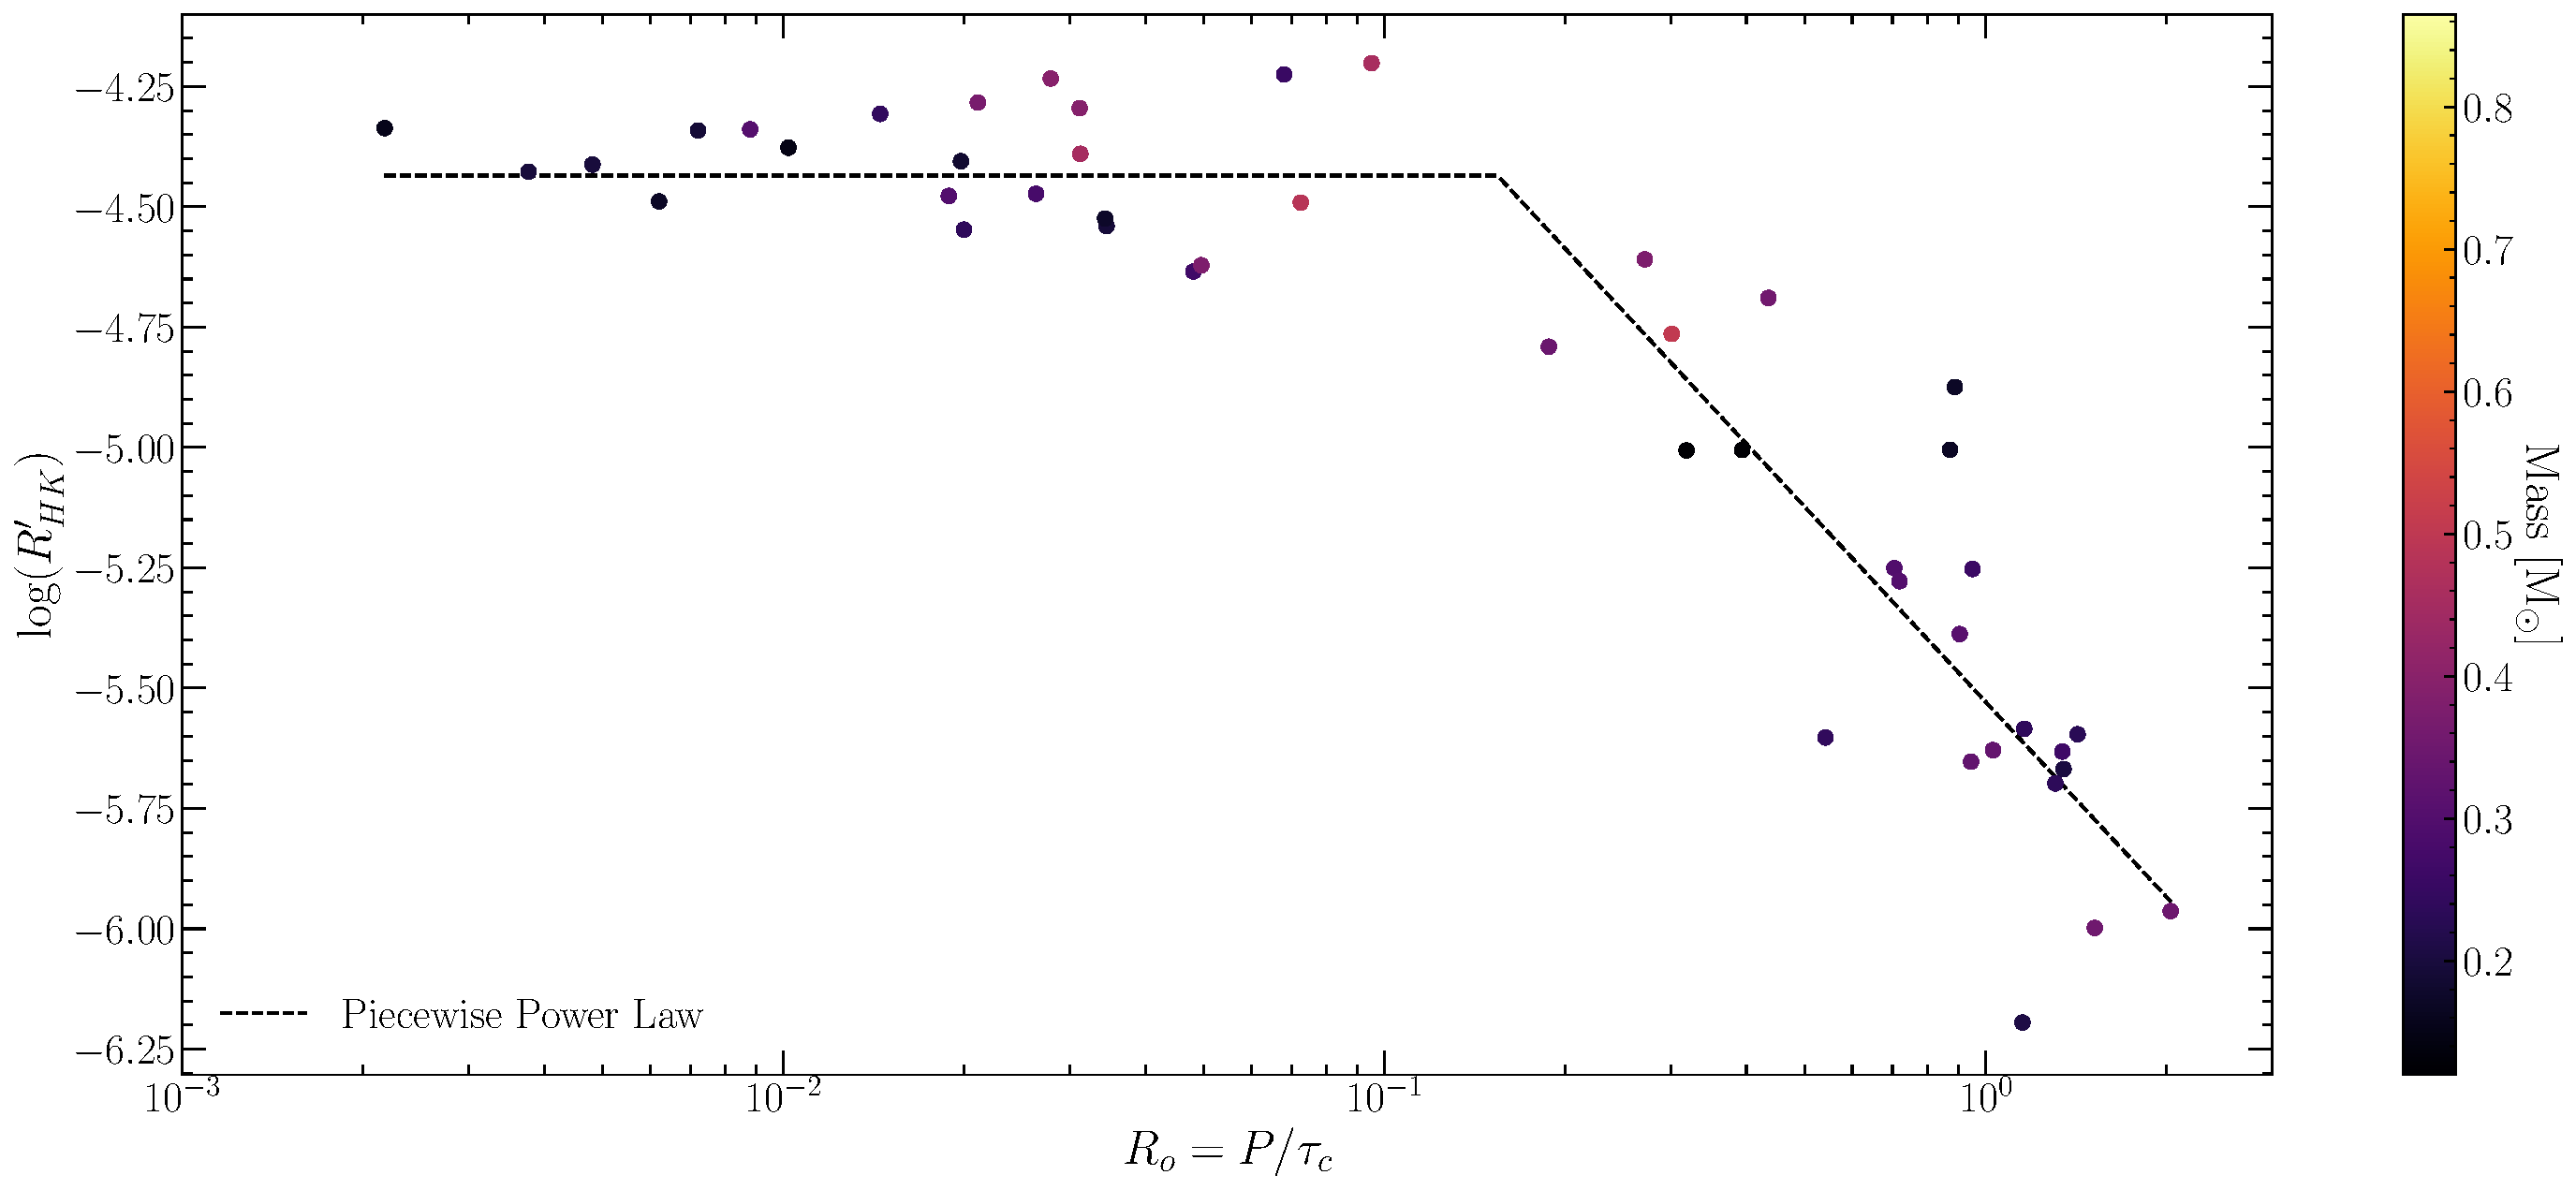
\includegraphics[width=0.9\textwidth]{figures/magActivity/RpHKvsR0_MC_justThisPaper.pdf}
	\caption{Rotation activity relation from this work. The color axis gives
	each stars mass. The dashed line is the best fit to our data set.}
    \label{fig:RpHKvsRossbySelf}
\end{figure*}
\begin{figure*}
    \centering
    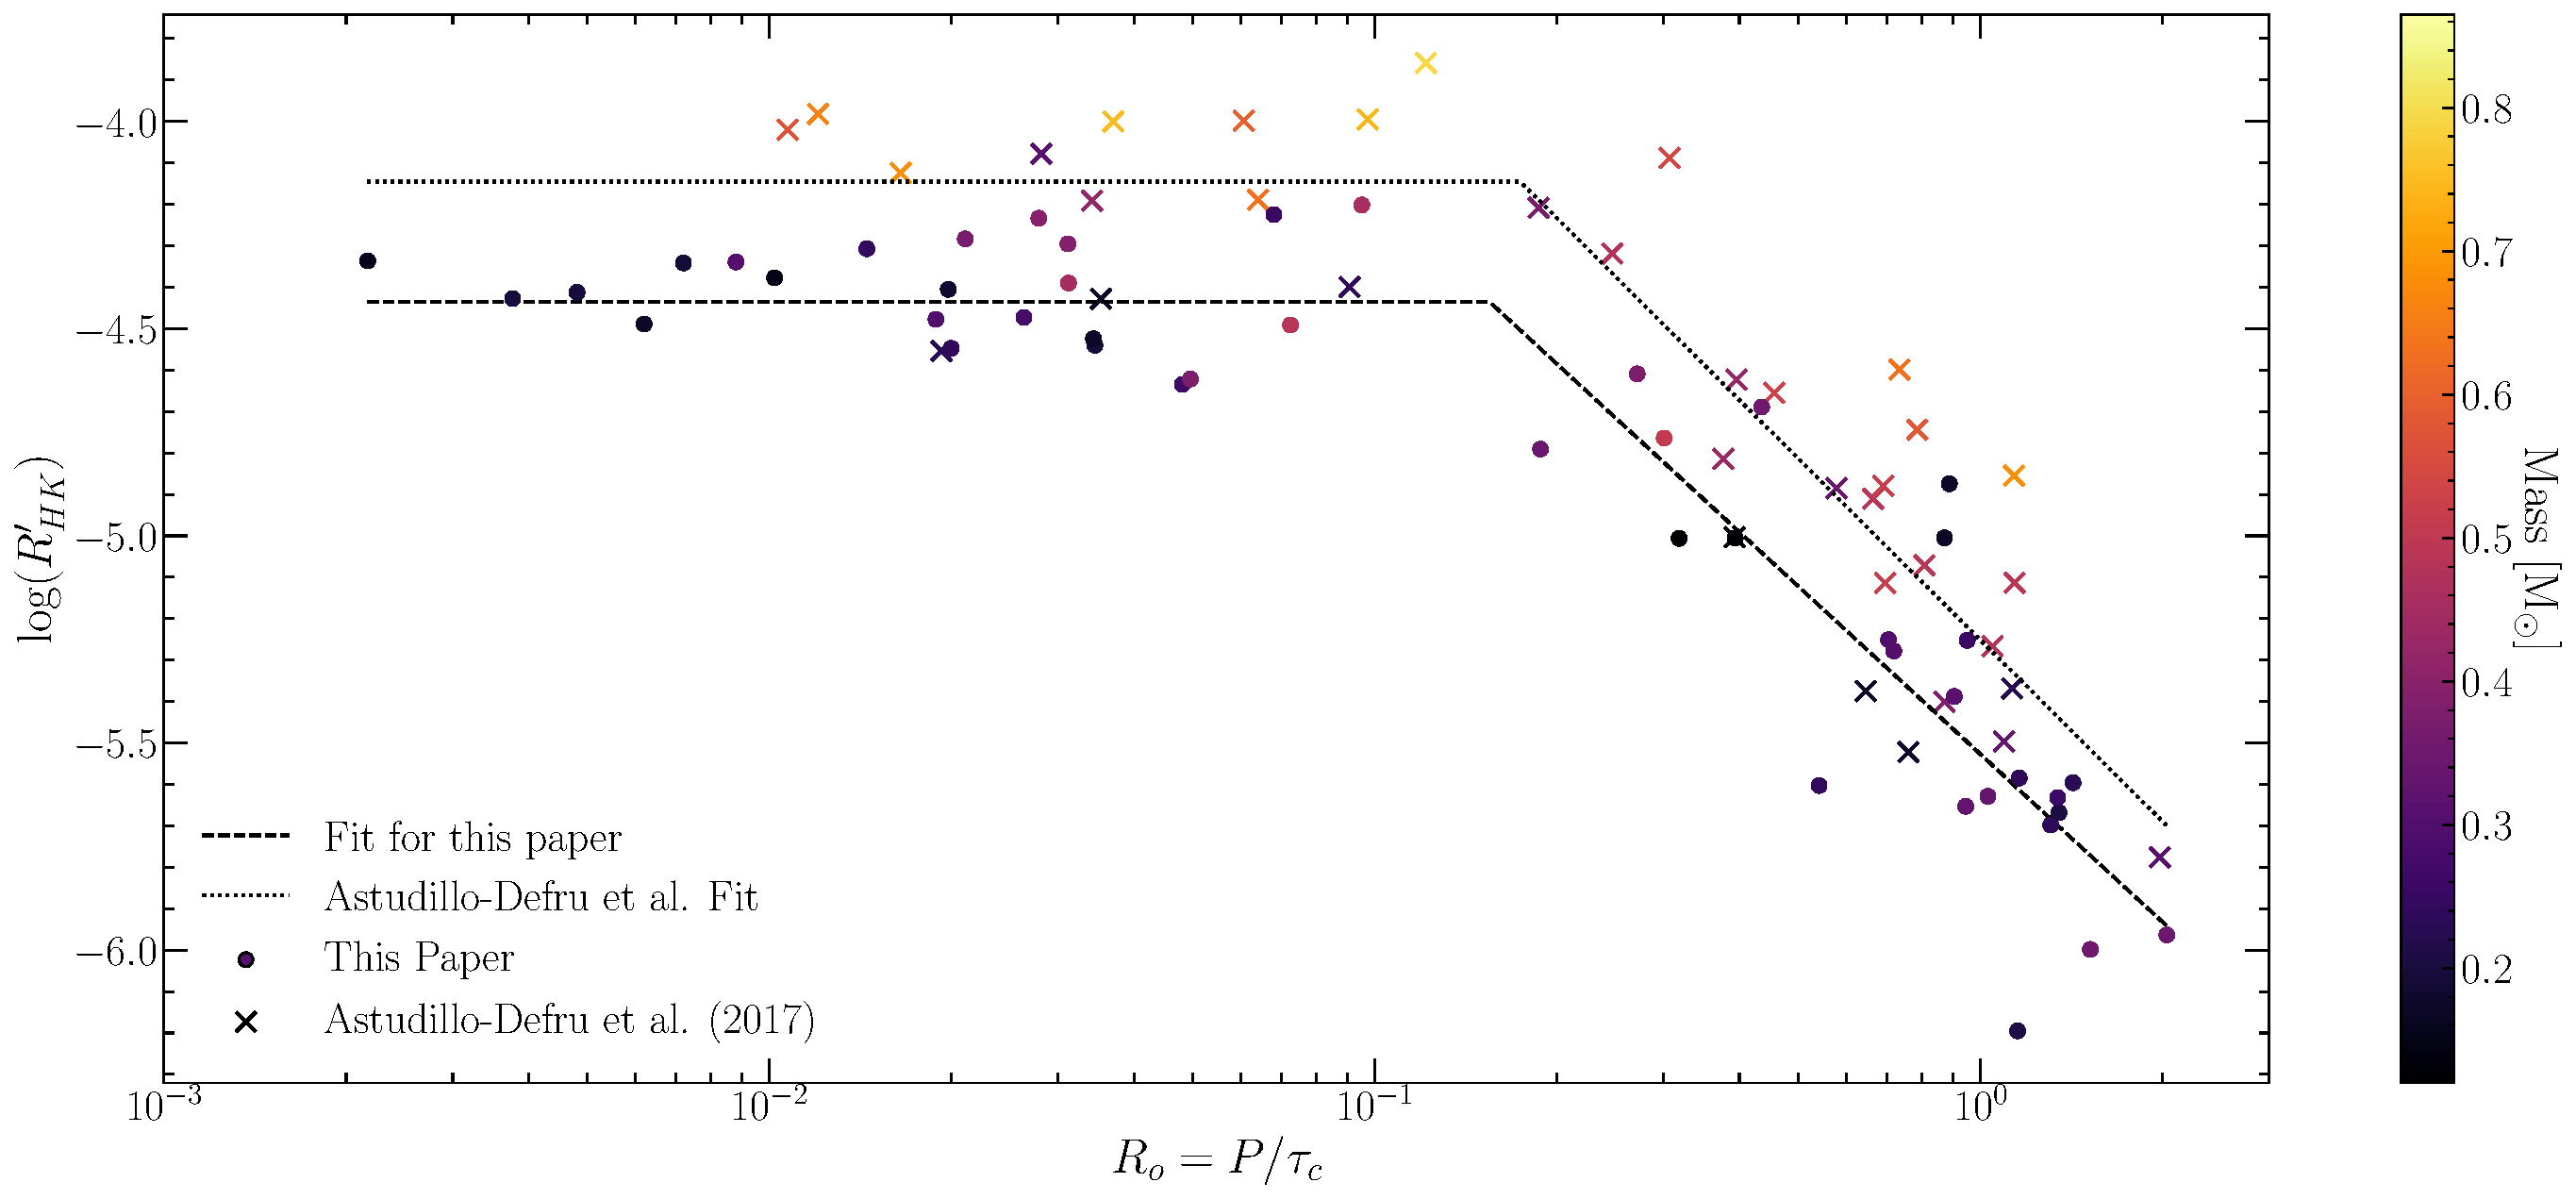
\includegraphics[width=0.9\textwidth]{figures/magActivity/RpHKvsR0_MC.pdf}
	\caption{Rotation activity relation for both our work and \citet{Def17}.
	The dotted line is the best fit to the re-derived rotation-activity
	relation from \citet{Def17}.  Note that targets from \citet{Def17} are
	systematically higher than targets presented here as a consequence of the
	range in mass probed by the samples.}
    \label{fig:RpHKvsRossbyDef}
\end{figure*}
\begin{figure*}
    \centering
    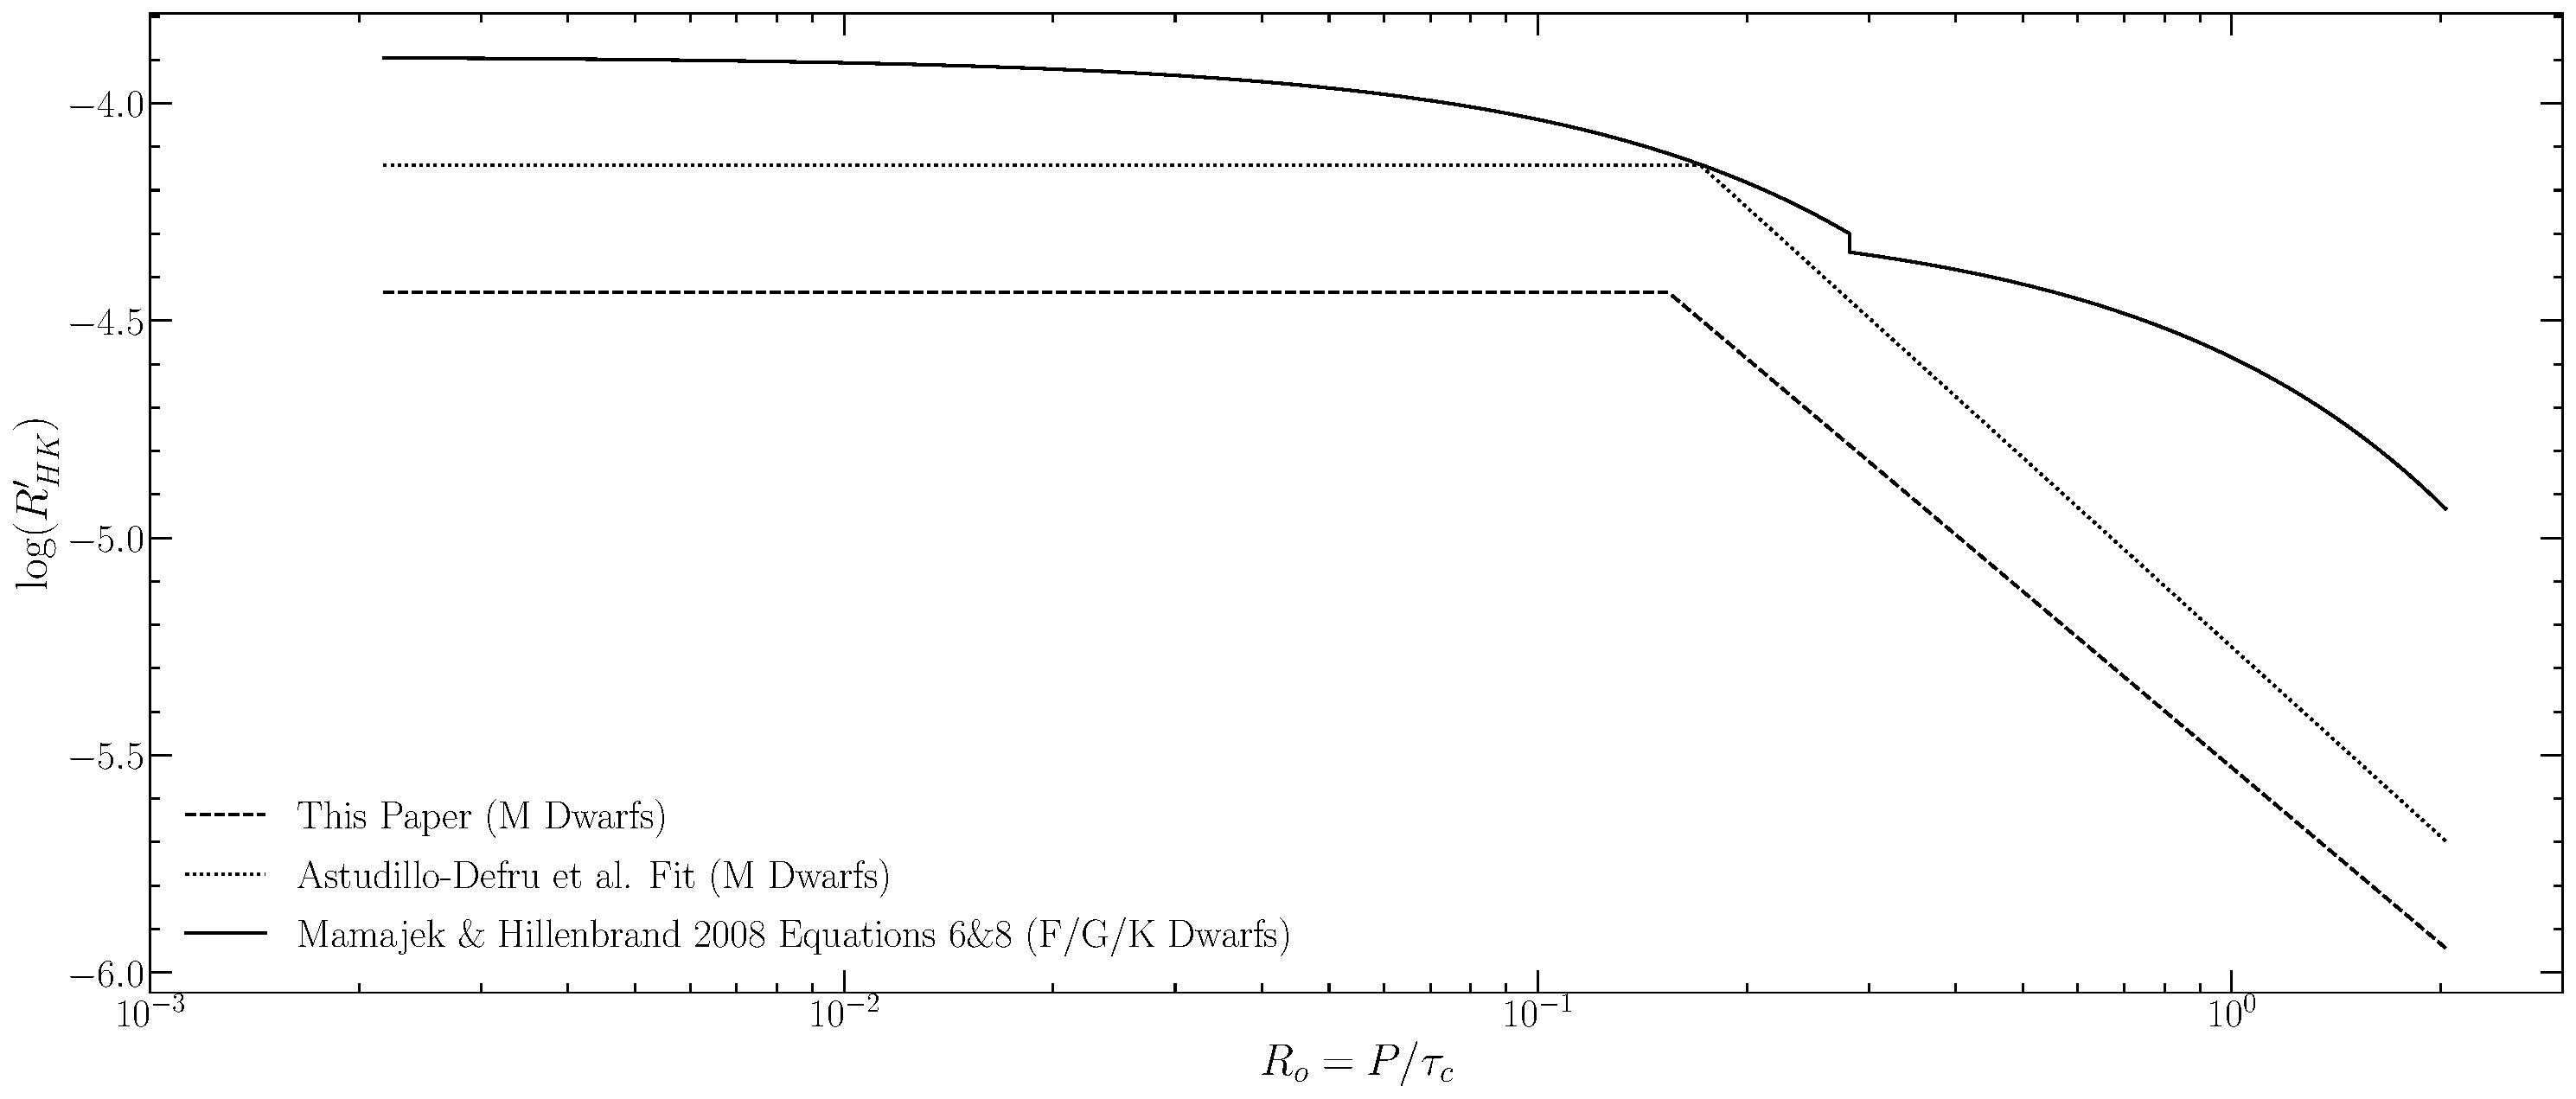
\includegraphics[width=0.9\textwidth]{figures/magActivity/RpHKvsR0_MC_fits.pdf}
	\caption{Derived rotation-activity curves from this work, \citet{Def17} and
	\citet{Mamajek2008}. Note both that \citet{Mamajek2008} focuses their work
	on earlier spectral classes and fits the rotation activity relation in
	linear space.}
    \label{fig:RpHKvsRossbyFits}
\end{figure*}

We find best fit parameters with one $\sigma$ errors:
\begin{itemize}
    \item $k = -1.347\pm 0.203$
    \item $Ro_{s} =  0.155\pm0.045$
    \item $\log(R_{s}) = -4.436\pm0.048$

\end{itemize}
\textbf{A comparison of the rotation activity derived in this work to those
from both \citet{Def17} and \citet{Mamajek2008} is presented in Figure
\ref{fig:RpHKvsRossbyFits}. For the 6 targets which do not have measured
rotational periods we include an estimate of $Ro$ and $p_{rot}$ in the machine
readable version of Table \ref{tab:finalData}. The convective overturn
timescale for one of these 6 targets (2MASS J13464102-5830117) can not be
inferred via Equation \ref{eqn:convectiveOverturn} as it lacks a V-K color
measurement. Instead, we infer $\tau_{c}$ via \citet{Wri18} Equation 6 (this
paper Equation \ref{eqn:ConvectiveOverturnTimeMass}) using mass. Similar to our
manner of inferring $\tau_{c}$ via color, when inferring $\tau_c$ via mass, we
adopt the larger of the two antisymmetric errors from \citet{Wri18}.}

\begin{equation}\label{eqn:ConvectiveOverturnTimeMass}
	\log_{10}(\tau_{c}) = 2.33\pm0.06 - 1.5\pm0.21\left(M/M_{\odot}\right) + 0.31\pm0.17\left(M/M_{\odot}\right)^{2}
\end{equation}

\textbf{Note that $R'_{HK}$ for one of six of these targets (2MASS
J15165576-0037116) is consistent to within 1$\sigma$ of the saturated value;
therefore, the reported $Ro$ for this target should only be taken as an upper
bound. The remaining five targets have measured $R'_{HK}$ values consistent
with the unsaturated regime. Estimated periods are consistent with previous
constraints. Of the six stars, two were listed as non-detections in
\citet{Newton2018}, and the remaining four as uncertain (possible) detections.
Of the four classed as uncertain, 2MASS 12384914-3822527 and 2MASS
19204795-4533283 have candidate periods $>100$ days and non-detections of
H-alpha emission \citep{Hawley96}. These two stars and the two non-detections
have Ca II H\&K activity levels suggesting very long periods. 2MASS
13464102-5830117 has a candidate period of 45 days, and 2MASS 15165576-0037116
of 0.8 days, both consistent with their higher levels of Ca II H\&K emission.}

As a test of the proposed weak correlation between activity and rotation in the
``saturated'' regime \textbf{seen in some works \citep{Mamajek2008,
Reiners2014, Leh20, Med20} --- though not in others \citep{Wri11, Nunez2015,
Newton2017} --- }  we fit a second model whose power law index is allowed to
vary at $Ro < Ro_{s}$. \textbf{We find a saturated regime power law index of
$-0.052\pm0.117$,} consistent with 0 to within 1$\sigma$. \textbf{Moreover,}
all other parameter for this model are consistent to within one $\sigma$ of the
nominal  parameters for the model where the index is constrained to 0 below
$Ro=Ro_{s}$. \textbf{We can constrain the slope in the saturated
regime to be between -0.363 and 0.259 at the $3\sigma$ confidence level.
Ultimately, we adopt the most standard activity interpretation, a
fully-saturated regime} at $Ro < Ro_{s}$. 

\textbf{We investigate whether our lack of detection of a slope for $Ro <
Ro_{s}$ is due to the limited number of observations in that region when
compared to other works \citep[e.g.][93 targets $Ro < Ro_{s}$]{Med20} through
injection and recovery tests. We inject, fake, rotation-activity measurements
into the saturated regime with an a priori slope of -0.13 --- the same as in
\citeauthor{Med20}. These fake data are given a standard deviation equal to the
standard deviation of our residuals ($12\%$). We preform the same MCMC model
fitting to this new data set as was done with the original dataset multiple
times, each with progressively more injected data, until we can detect the
injected slope to the three sigma confidence level. Ultimately, we need more
than 65 data points --- 43 more than we observed in the saturated regime --- to
consistently recover this slope. Therefore, given the spread of our data we
cannot detect slopes on the order of what has previously been reported in the
literature.}

We observe a gap in rotational period \textbf{over a comparable range} to the
one presented in \citet{Newton2016} Figure 2. Namely, that M-dwarfs are
preferentially observed as either fast or slow rotators, with a seeming lack of
stars existing at mid rotational periods. This period gap manifests in the
Rossby Number and can be seen in Figure \ref{fig:RpHKvsRossbyDef} as a lack of
our targets near to the knee-point in the fit. \textbf{This period gap likely
corresponds to that seen by \citet{Browning2010}, who found a paucity of M
dwarfs at intermediate activity levels in Ca II H\&K and note the similarity to
the Vaughn-Preston gap established in higher mass stars \citep{vaughan1980}.
\citet{Magaudda2020} also identify a double-gap in x-ray activity for stars in
the unsaturated regime; it is not clear that the gap we see is related.} As a
consequence of this period gap, there exists a degeneracy in our data
between moving the knee-point and allowing the activity level to vary in the
saturated regime.  In the following, we adopt the model of a fully saturated
regime.

We wish to compare our best fit parameters to those derived in \citet{Def17};
however, the authors of that paper do not fit the knee-point of the
rotation-activity relation. They select the canonical value for the rotational
period separating the saturated regime from the unsaturated regime ($P_{rot,s}
= 10$ days) and use a fixed convective overturn timescale ($\tau_{c} = 70$
days). To make our comparison more meaningful we use the $P_{rot}$ and $V-K$
colors presented in \citet{Def17} to re-derive $Ro$ values using $\tau_{c}$
\citep{Wri18}. Doing this for all targets presented in \citet{Def17} Table 3
and fitting the same piecewise power law as before, we find best fit parameters
of $Ro_{s} = 0.17\pm0.04$, $\log(R_{s}) = -4.140\pm0.067$, and
$k=-1.43\pm0.21$. Compared to the best fit parameters for our data, $Ro_{s}$
and the unsaturated regime's index, $k$, are consistent to within one sigma,
while the saturated value, $R_{s}$, differs. 

The mass ranges of our respective samples explain the differences in saturation
values between our work and that of \citet{Def17}. Our work focuses on
mid-to-late M-dwarfs and includes no stars above a mass of $0.5$ M$_{\odot}$
(Figure \ref{fig:massDistribution}).  \textbf{The strength of Ca II H\&K
emission is known to decrease as stellar mass decreases \citep{Schrijver1987,
Rauscher2006, Hou17}. As \citet{Rauscher2006} note, this is the opposite as the
trend seen in H-alpha; the latter primarily reflects the increasing length of
time that lower M dwarfs remain active and rapidly rotating \citep{West2015,
Newton2016}.}

\textbf{A mass dependence can be seen in Figure 10 in \citet{Def17}, consistent
with expectations from the literature.} If we clip the data from \citet{Def17}
Table 3 to the same mass range as our data-set ($M_{*} < 0.5M_{\odot}$) and fit
the same function as above, we find that all best fit parameters are consistent
to within one sigma between the two data-sets. 

\begin{figure}
    \centering
    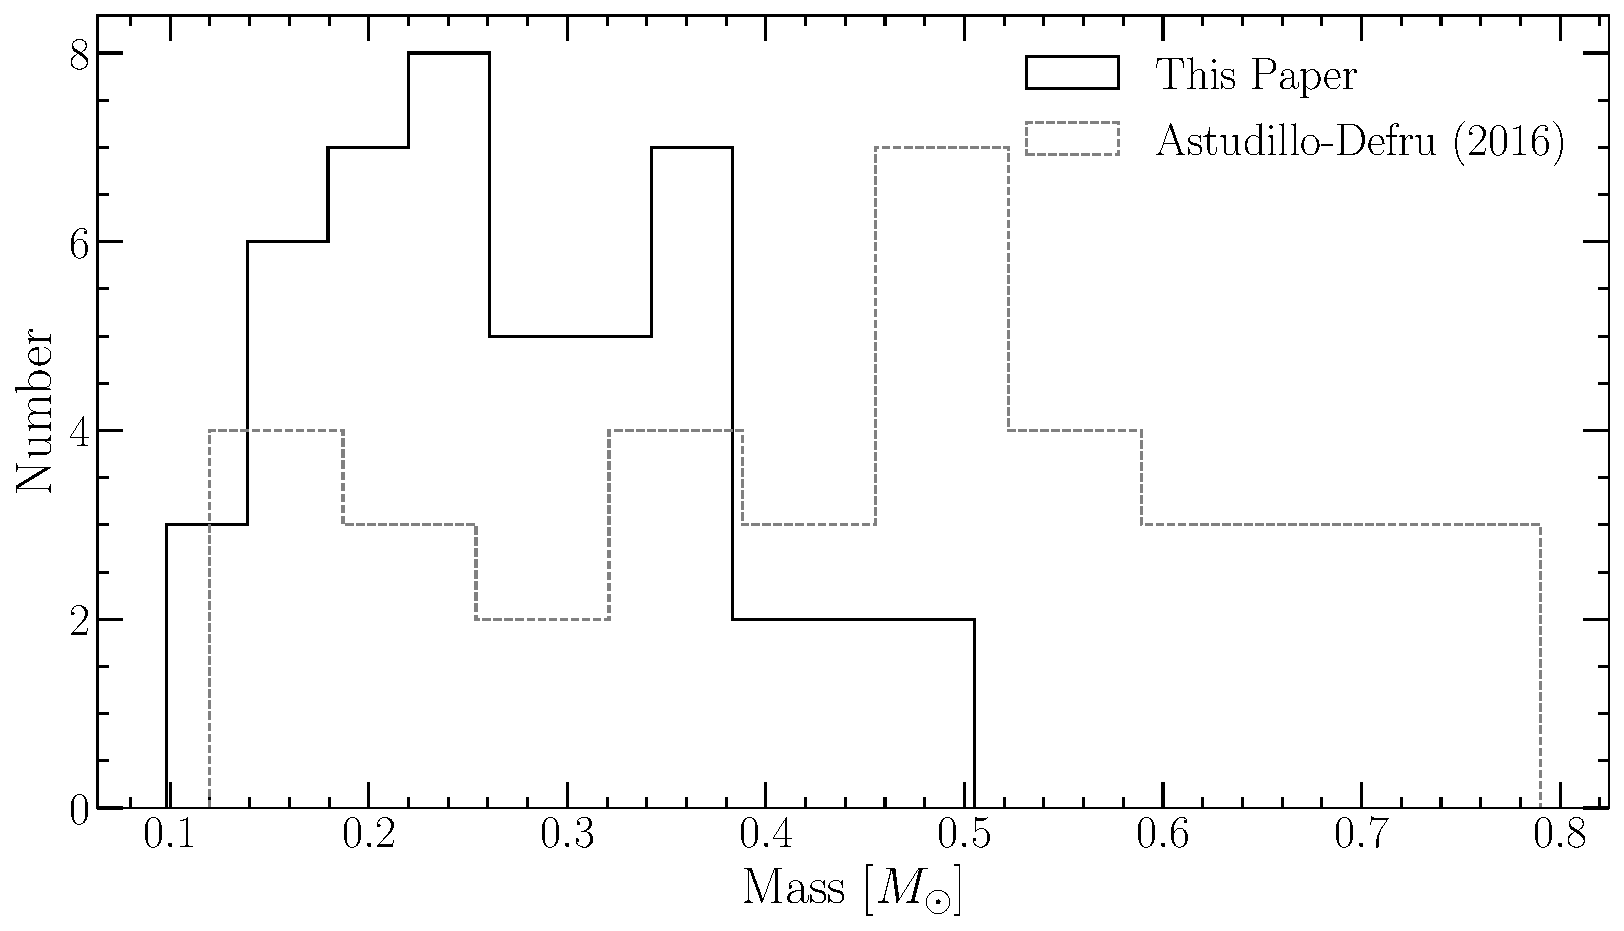
\includegraphics[width=0.47\textwidth]{figures/magActivity/B2020vsAD2016_Masses.pdf}
	\caption{Distribution of masses between our sample and the sample presented
	in \citet{Def17}. Note how the two studies have approximately the same
	sample sizes; however, our sample is more tightly concentrated at lower
	masses \textbackslash later spectral classes.}
    \label{fig:massDistribution}
\end{figure}

We also compare our best fit $Ro_{s}$ to both those derived in
\citet{Newton2017} using $H_{\alpha}$ as an activity measure and those derived
in \citep{ Wri18, Magaudda2020} using $L_{X}/L_{bol}$ as an activity measure.
Works using $L_{X}/L_{bol}$ identify a similar, yet not consistent to within
one sigma result for $Ro_{s}$; while, the value of $k$ we find here is
consistent between all four works. Therefore, we find similar results not only
to other work using the same activity tracer, but also a power-law slope that
is consistent with work using different tracers. 
